\documentclass{article}
\usepackage{graphicx} % Required for inserting images
\graphicspath{ {./images/} }
\usepackage[square,numbers]{natbib}
\usepackage[letterpaper,top=2cm,bottom=2cm,left=3cm,right=3cm,marginparwidth=1.75cm]{geometry}
\usepackage{hyperref}

\bibliographystyle{dinat}


\begin{document}


\title{Unit 13}
\author{Chris Hadden}
\date{}
\maketitle

\section{P3 Understand the use of Social Media in business}

\section{Introduction on the use of Social Media in business}
As a valued member of Titanica Media we want you to be able to understand what it is and how we do it. This report will hopefully get you up to speed quickly with our ethos and how we go about business.

When most of our clients want to work with us, they will know from our previous campaigns that they can trust us and that their brand or product will get the boost that they are looking for.

\section{How social media can be used to gather data}
\subsection{Research}
\subsubsection{Primary data}
Primary data is data that in Titanica Media collect ourselves, it's something that we have planned for and we know what we want and what we want to do with the data.
Collecting primary data can be an expensive task so we tend to only do it when there is something we specifically want to find out and there's no other way to get the data.

\subsubsection{Secondary data}
Secondary data is data that was gathered by someone else. This type of data is a lot cheaper the collecting Primary data, but it may not be exactly what we are looking for. Most general data like population density can be found for free, but more specialist Secondary data can be costly. Also as the data is in the public domain other companies may already be using it anc that may reduce it's value to us.

\subsection{Data as a resource}
At Titanica Media we see social media as resource, a resource that we can use to gather data about marketing from.

There are many aspects to gathering social media data that you need to be aware of, some of these are:
\begin{itemize}
\item Data Management: DAMA, a data management professional organization has defined data management as "The planning, execution and oversite of policies, practices and projects that acquire, control, protect, deliver, and enhance the value of data and information assets." \cite{dama}\\
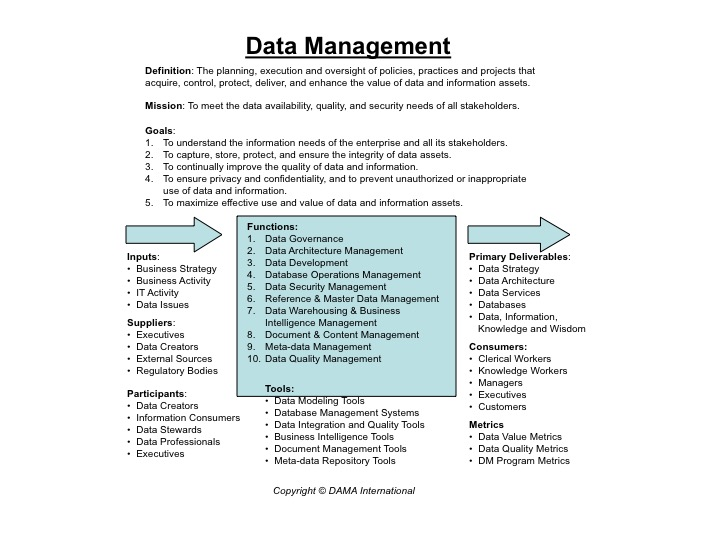
\includegraphics[scale=0.5]{datamanagement} \\
Typically a data management team needs to be setup to deal with how data is organised and stored. 
\item Sources of Data: This can be data gathered from social media about users or could be gathered from users web cookies or many other inventive ways of gathering it.
\item Collection of Data:How we collect data will depend on relationship with the source of data. We can pay for reports and tools supplied by social media or we can scrape basic metrics that everyone has access to. It depends on what data you need.
\item Analysis of Data: Automated Data Mining is the process of processing all our data collections, which is usually numerous. There is a semantic difference in the meaning ot pattern and trend here. A pattern will describe the layout of responses and a trend is defined over time.
\item Sale of Data: Data is an asset. It can be sold for gain to the company. The extent to which we may gather data is limited by the Data Protection Act in the UK.

\end{itemize}



\bibliography{bibliography}

\end{document}

